\section{Motivation and Research Overview}
\label{sec:motivation}

As discussed earlier, there are  three key aspects to the \ArchName vision for
\DC networks: {\em flexibility}, {\em wireless}, and the use of {\em free-space
optics}.  We argue why  each of these aspects is needed before providing an
overview of our proposed  research.




 

\subsection{Flexibility reduces infrastructure needs}  

 Measurement studies show that  \DC traffic exhibits low utilization coupled
with hotspots of inter-rack activity with  a few ``heavy''
flows~\cite{flyways,cthrough,vl2}.  In light of this, traditional {\em static}
\DC designs turn out to be extreme points in the  cost-performance tradeoff.
Fat-tree~\cite{XXX} like solutions that provide full bisection bandwidth are
overprovisioned and lead to low link utilization and high cost.  On the other
hand, conventional  leaf-spine architectures are low cost but suffer poor
performance as many links are oversubscribed~\cite{XXX}.    As observed in
prior work~\cite{},
  these measurement studies naturally suggest that a {\em flexible}
\DC topology can potentially eliminate the need for
overprovisioning~\cite{XXX}.   


\begin{wrapfigure}{r}{0.4\textwidth}
\captionsetup[subfloat]{captionskip=-15pt}
\vspace{-2.1cm}
\subfloat[Long-lived flows]
{
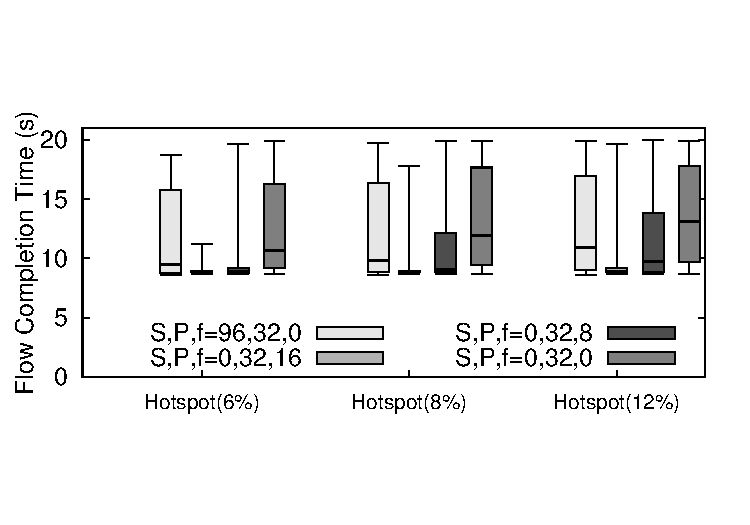
\includegraphics[width=200pt]{zafar_htsim/fct_long_flows_gray.pdf}
} \vspace{-0.7cm} \\
\subfloat[Short-lived flows]
{
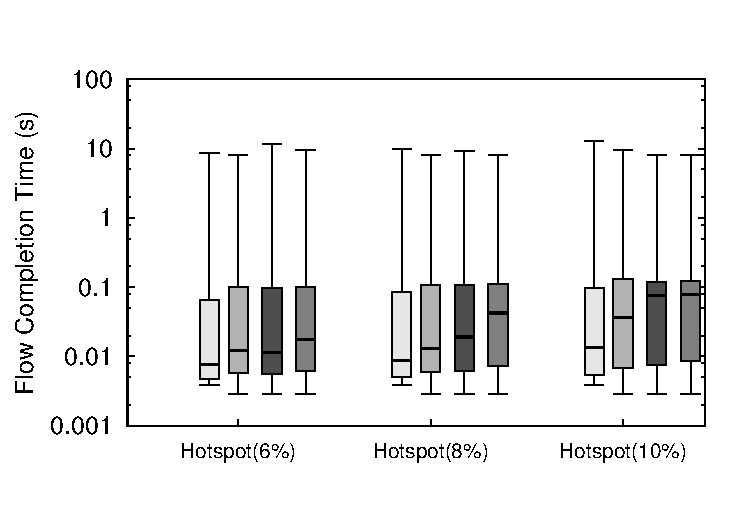
\includegraphics[width=200pt]{zafar_htsim/fct_short_flows_gray.pdf}
}
\caption{A flexible \DC provides similar or better performance relative to overprovisioned networks with much less infrastructure.}
\label{fig:flexibility}
\end{wrapfigure}



To provide the basis for this intuition, we consider an abstract model of a \DC
with $\NumRacks$ \ToR switches  and  $\NumNonToR$ ``core'' switches that
transit traffic between \ToR switches.  Each rack has $\NumMachinesPerRack$
servers and   each  switch (\ToR and core) has $\NumPortsPerToR$ ports. For the
\ToR switches, $\NumMachinesPerRack$ ports connected to the machines, and
$\NumPortsPerToR - \NumMachinesPerRack$ for inter-rack connections.
Furthermore, out of the $\NumPortsPerToR - \NumMachinesPerRack$ inter-rack
ports, suppose $\DegreeFlex$ can be {\em flexibly} rewired. For the non-\ToR
switches, all $\NumPortsPerToR$ ports are connected to other switches.  Now,
for a given $\NumRacks$,  $\NumMachinesPerRack$, and $\NumPortsPerToR$
determined by technology or deployment constraints,  we can define a broad
spectrum of \DC  designs by specifying the 3-tuple $\langle \NumNonToR,
\NumPortsPerToR, \DegreeFlex \rangle$.  For instance, with $\NumPortsPerToR = 2
\times \NumMachinesPerRack$ that is typical of \DC designs today,   $\langle
1.5\NumRacks, 2 \NumMachinesPerRack,  0 \rangle$ corresponds to traditional
{\em static} fat-tree designs and  $\langle 0,  2 \NumMachinesPerRack,
\NumMachinesPerRack \rangle$ captures  an extreme \ArchName point  with no
``core'' switches and full flexibility.  


 Of course, for a given $\langle \NumNonToR, \NumPortsPerToR,\DegreeFlex
\rangle$, we also need to specify the topology created by the ``static'' and
``dynamic'' links.  Rather than explore all possible graph structures for the
{\em static} links, for brevity we only consider {\em random regular graphs}
building on the observation that they provide close-to-optimal
performance~\cite{XXX}.  Thus, we randomly wire the ``static'' links between the
\ToR and  non-\ToR switches.  Based on our preliminary work, we use a greedy
algorithm for the dynamic links where we simply add ``short-cut'' links between
racks with the highest inter-rack demands~\cite{hotnets}.


 Given this abstraction, we evaluate the performance of different \DC designs
by custom extensions to the {\tt htsim} packet-level simulator~\cite{htsim}.
Building on the prior \DC measurements, we consider realistic \DC traffic
workloads~\cite{XXX}, wtih  a baseline {\em uniform} traffic matrix between
racks consisting of short-lived flows with an average size of \plsfill. We
augment this baseline with ``elephant'' or large flows between a subset of
``hotspot'' racks with an average size of \plsfill. In this configuration, {\tt
Hotspot-X} refers to X\% of the rack-pairs having elephant flows. 


 As an illustrative example, we consider the scenario with $\NumRacks$=64 racks
with $\NumPortsPerToR$=32 and $\NumMachinesPerRack$=16 in
Figure~\ref{fig:flexibility} with each link having \plsfill~Gbps.  The result
shows a box-and-whiskers plot with the min, max, and quantiles of the the flow
completion times  for different \DC designs.  Here, $\langle 96,32,0 \rangle$
is a  static regular random graph that provides full-bisection bandwidth with
$\NumNonToR=96$ ``core'' switches.  We consider three  flexible designs with
$\DegreeFlex$ =  0, $\NumPortsPerToR - \NumMachinesPerRack = 16$ (i.e., fully
flexible), and $ \frac{\NumPortsPerToR - \NumMachinesPerRack}{2} = 8$.   The
key takeaway here is that  flexible designs achieve near-optimal or better
performance with significantly less infrastructure requirements.  Specifically,
the $\langle 0,*,* \rangle$ configurations  uses 1.5$\times$ fewer switches and
edges, but achieve  very good performance.  For instance, $\langle
0, 8 \rangle$ configuration increases the  median and 75\%-ile of the flow
completion time for short flows only by  \plsfill and \plsfill respectively but
{\em decreases} that for long flows  by \plsfill and \plsfill respectively. We
have also confirmed that these results qualitatively hold for other  \DC
configurations as well; e.g., with $\NumRacks=$256 racks and
$\NumPortsPerToR$=32 the corresponding improvements are \plsfill.



 %talk about cabling,  power cooling  
\subsection{Case for all-wireless and FSO} 

\myparaq{Why wireless} To realize  a flexible inter-rack fabric, conceptually we need
a reconfigurable ``patch-panel''  between  pairs of racks~\cite{sdnpatch}. Of
course, such a big-switch abstraction is infeasible: (1) it requires very high
fanout ($\NumRacks \times \DegreeFlex$, where $\NumRacks$ is the number of
racks and $\DegreeFlex$ is the number of flexible links at each ToR) and
backplane  switching capacity; and (2)
the  cabling complexity  would be prohibitive and create
operational overheads w.r.t failures, and cooling/airflow
considerations~\cite{XXX}.  For similar reasons, traditional optical
 switching is also not viable.  Finally, this giant switch 
  introduces a single-point of failure~\cite{osa,proteus,helios}. 
 To avoid the need for such a massive switch, 
 we turn to  {\em reconfigurable wireless} links between the  ToR switches.\footnote{Note that we are not proposing a fully wireless data center~\cite{cornell}; our focus is on the ``inter-rack'
fabric.}


%% wireless is not good enough hence fso
\myparaq{Why FSO} The seemingly natural  solution then is 
 traditional radio-frequency (RF) wireless technologies (e.g., 60GHz).
Unfortunately, these  have  many fundamental performance 
limitations: (1)  RF links produce a
large interference footprint due to a wide beamwidth
~\cite{XXX}. \samir{This blames one paper only. This does
not argue why we are discounting every form of RF. Recall the comment from
hotnets reviewer. I can fix this. But the real argument is somewhat involved -- more than a oneliner.}  (2) The beam-steering  technologies
 to implement flexibility are  slow and
inaccurate~\cite{3db} and may additionally increase the interference
footprint~\cite{phased-arrays-rf}; \samir{Need to rephrase, overly sweeping.} 
and (3) The data rates of RF links fall off
rapidly with distance~\cite{3db} and the use 
 of  higher transmit power to increase the range 
 will increse interference and is limited by regulations~\cite{}.
To overcome these limitations, we leverage a somewhat non-standard wireless 
technology---free-space optics (FSO) that uses modulated visible or
infrared (IR) laser beams~\cite{kedar}.\footnote{Unlike traditional optical
links, the laser beam in FSO is not enclosed in a glass fiber, but transmitted
through the air (and hence  ``free space'').}  
 We elaborate on the advantages of FSO vs.\ RF in Section~\ref{sec:fso}.





\subsection{Architecture and Proposed Research}
 
\begin{wrapfigure}{r}{0.4\textwidth}
\label{fig:benefits}
\vspace{-0.6cm}
\centering
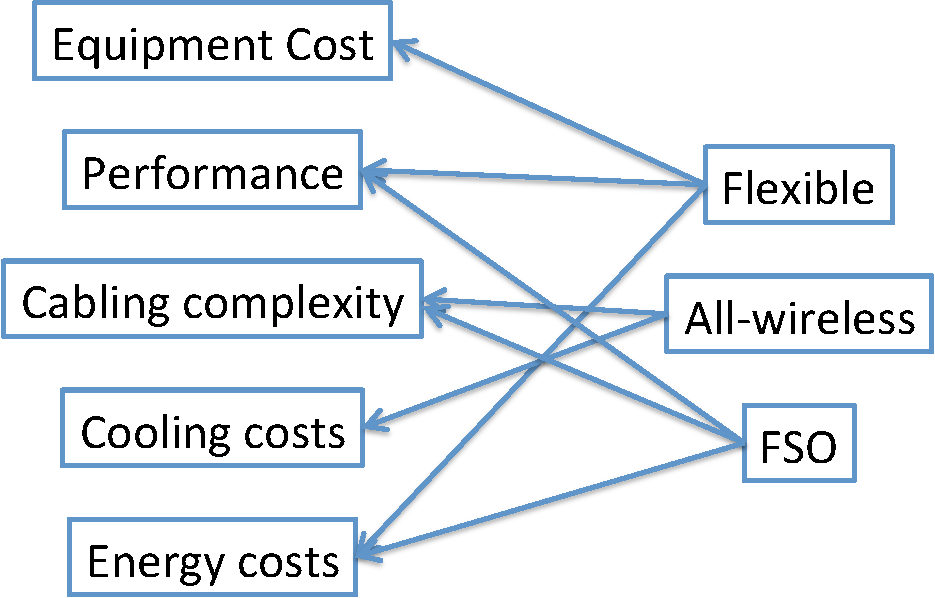
\includegraphics[width=150pt]{PPTFigs/benefitidea.pdf}
\caption{ Key ideas underlying the \ArchName vision and
  how they benefit different 
 of \DC datacenter considerations from Section~\ref{sec:intro}}
\label{fig:benefits}
\vspace{-0.4cm}
\end{wrapfigure}


%% benefits
Combining the above arguments leads us to the architecture   
in Figure~\ref{fig:vision}.  We eliminate the need for a wired backbone network
and rely on a reconfigurable FSO-based wireless fabric.  Each \ToR switch is
equipped with a  pre-specified number of FSO devices and  each FSO device
assembly is capable of precise and fast steering to connect to  target
 FSO devices in other \ToRs. 
  To establish an {\em obstruction-free} optical path, the space
 above the racks is a natural choice for laser propagation as this
 space is roughly free from obstruction~\cite{samirpic}.  The FSO
 transceivers will be anchored on the top of the rack and connected to
 the ToR switch.  \blue{To ensure that the devices themselves do not
   obstruct each other, we propose use of ceiling mirrors as
   in~\cite{3db} (and possibly additional mirrors on the beam path).}

 The \DC management layer  intelligently
reconfigures these devices  to adapt to  changing network requirements.
 Figure~\ref{fig:benefits} summarizes  how the three key aspects of
\ArchName---flexibility, all-wireless, and use of FSOs--- benefit different
considerations of \DC network design: (1) Flexibility  ensures high-performance
with lower cost  and  enables energy reduction~\cite{}; (2) A wireless  fabric
eliminates concerns about cabling complexity and  interference with
cooling~\cite{hpcabling}; and (3) Using FSOs eliminate performance concerns for
a wireless network that might arise from range and  interference constraints. 

While \ArchName is not the first architecture to explore a {\em flexible} \DC
architecture, we highlight  two key aspects of  that make it significantly
different from  prior work on optical or wireless augmentation. First, we are
eliminating the need for a wired core and core switches.  Second,  the use of
FSO-based inter-rack links provides a better alternative to existing RF
wireless or  optical solutions.



%% roadmap
\subsection{Preliminary work:  Cost vs.\ performance tradeoff}

\begin{wraptable}{r}{0.4\linewidth}
\vspace{-0.8cm}
\begin{footnotesize}
\begin{center}
\begin{tabular}{c|c|l}
Architecture & Cost (\$) &  Per-server \\ & & throughput \\   \hline % \hline
 \ArchName (16) & 18.1M  & 1.7 Gbps\\    
3D Beamforming~\cite{} & 17.1M  & 1.1 Gbps\\
Jellyfish~\cite{} 1Gbps & 13M & 1 Gbps\\
Jellyfish 2 Gbps & 26M  & 2 Gbps \\ 
 \ArchName (48) & 37.8M  & 8.5 Gbps \\ 
Fattree/Jellyfish 10Gbps & 57M  & 10 Gbps
\end{tabular}
\end{center}
\end{footnotesize}
\vspace{-0.4cm}
\caption{Cost and performance of \ArchName vs.\ state-of-art proposals for a 512 rack, 48 machines/rack 
 \DC}
\vspace{-0.2cm}
\label{table:cost}
\end{wraptable}

In a preliminary position paper~\cite{hotnets}, we analyzed the
cost-performance tradeoff of candidate \DC architectures for a 512 rack \DC with 48 machines/rack,
  based on publicly available cost projections. Specifically, we consider  full-bisection bandwidth
networks such as FatTree~\cite{XXX} and Jellyfish~\cite{XXX} and the
3D-Beamforming architecture using 60Ghz wireless and ceiling
mirrors~\cite{XXX}.\footnote{We don't consider the all-wireless architecture
of~\cite{cornell} because  it has worse cost-performance tradeoffs; e.g., for
24k machines it costs $\approx 50M$ but only achieves 300-400 Mbps
per-server~\cite{cornell}.} FatTree/Jellyfish-Y Gbps 
 refers to a network with bisection bandwidth  of Y~Gbps, with Y=1,2, and 10.
Here, \ArchName($X$) refers to a hypothetical realization of the \ArchName
vision with $X$ FSO devices on each \ToR switch. 

 We assume that a 64-port 10Gb \ToR switch costs
\$27K: \$11K for the bare switch~\cite{64switch}, and \$16K for 64 10Gbps
optical transceivers at \$250 each~\cite{sfp}. We assume that a 48-port 1Gb
switch costs \$5000~\cite{48-switch-cost}, and each 60GHz radio costs \$1000.
We assume a hypothetical steerable FSO device can be constructed with a total
cost of roughly \$750 (see Section~\ref{sec:fso}).   We conservatively ignore
cabling costs for the wired core for FatTree, Jellyfish, and 3D-Beamforming.
Given the above assumptions, Table~\ref{table:cost} summarizes the cost and the
throughput that different \DC architectures offer based on our simulations.
 The result  shows that   \ArchName offers good cost-performance tradeoffs  w.r.t.\ state-of-art
solutions; e.g., close to 9~Gbps bisection bandwidth at much less cost
compared to a Fat-tree, and 90\% of the performance for 2~Gbps fat-tree at
70\% of the cost.


With this context,  we discuss the three broad research thrusts we need to
address to turn the benefits (Figure~\ref{fig:flexibility},\ref{fig:benefits})
into reality: (1) {\em feasibility of FSOs for \ArchName
(Section~\ref{sec:fso})},   (2) {\em foundations of flexible topology design
(Section~\ref{sec:topology})}, and  (3) {\em effective datacenter management
(Section~\ref{sec:system}).}


